%
% software.tex
%
% Copyright (C) 2021 by SpaceLab.
%
% TTC Documentation
%
% This work is licensed under the Creative Commons Attribution-ShareAlike 4.0
% International License. To view a copy of this license,
% visit http://creativecommons.org/licenses/by-sa/4.0/.
%

%
% \brief Software description chapter.
%
% \author Gabriel Mariano Marcelino <gabriel.mm8@gmail.com>
%
% \institution Universidade Federal de Santa Catarina (UFSC)
%
% \version 1.2.0
%
% \date 2021/01/16
%

\chapter{Software} \label{ch:software}

The beacon software is responsible to transmit periodic beacon signals, containing the satellite identification and a basic telemetry data.

To achieve it, this software communicates with other modules of the satellite (to acquire data to transmit in the beacon packets), controls the beacon's radio module and its antenna module.

It's written in C, using the Code Composer Studio IDE (Version 7.4.0). The radio module (Si4463 IC) is configured using the WDS (Version 3.2.11), a step-by-step tutorial is available as an apendix.

\section{Dependencies}

The beacon software is dependent of the following libraries:

\begin{itemize}
    \item NGHam: Used to generate and interpret the NGHam protocol packets (This library was modified for this firmware).
    \item DriverLib: Used to handle the internal peripherals of the MSP430F6659 uC.
\end{itemize}

\nomenclature{\textbf{HAL}}{Hardware Abstraction Layer.}

\section{Software Layers}

The figure \ref{fig:beacon-software-layers} describes the software layers of the beacon system.

\begin{figure}[!h]
	\begin{center}
		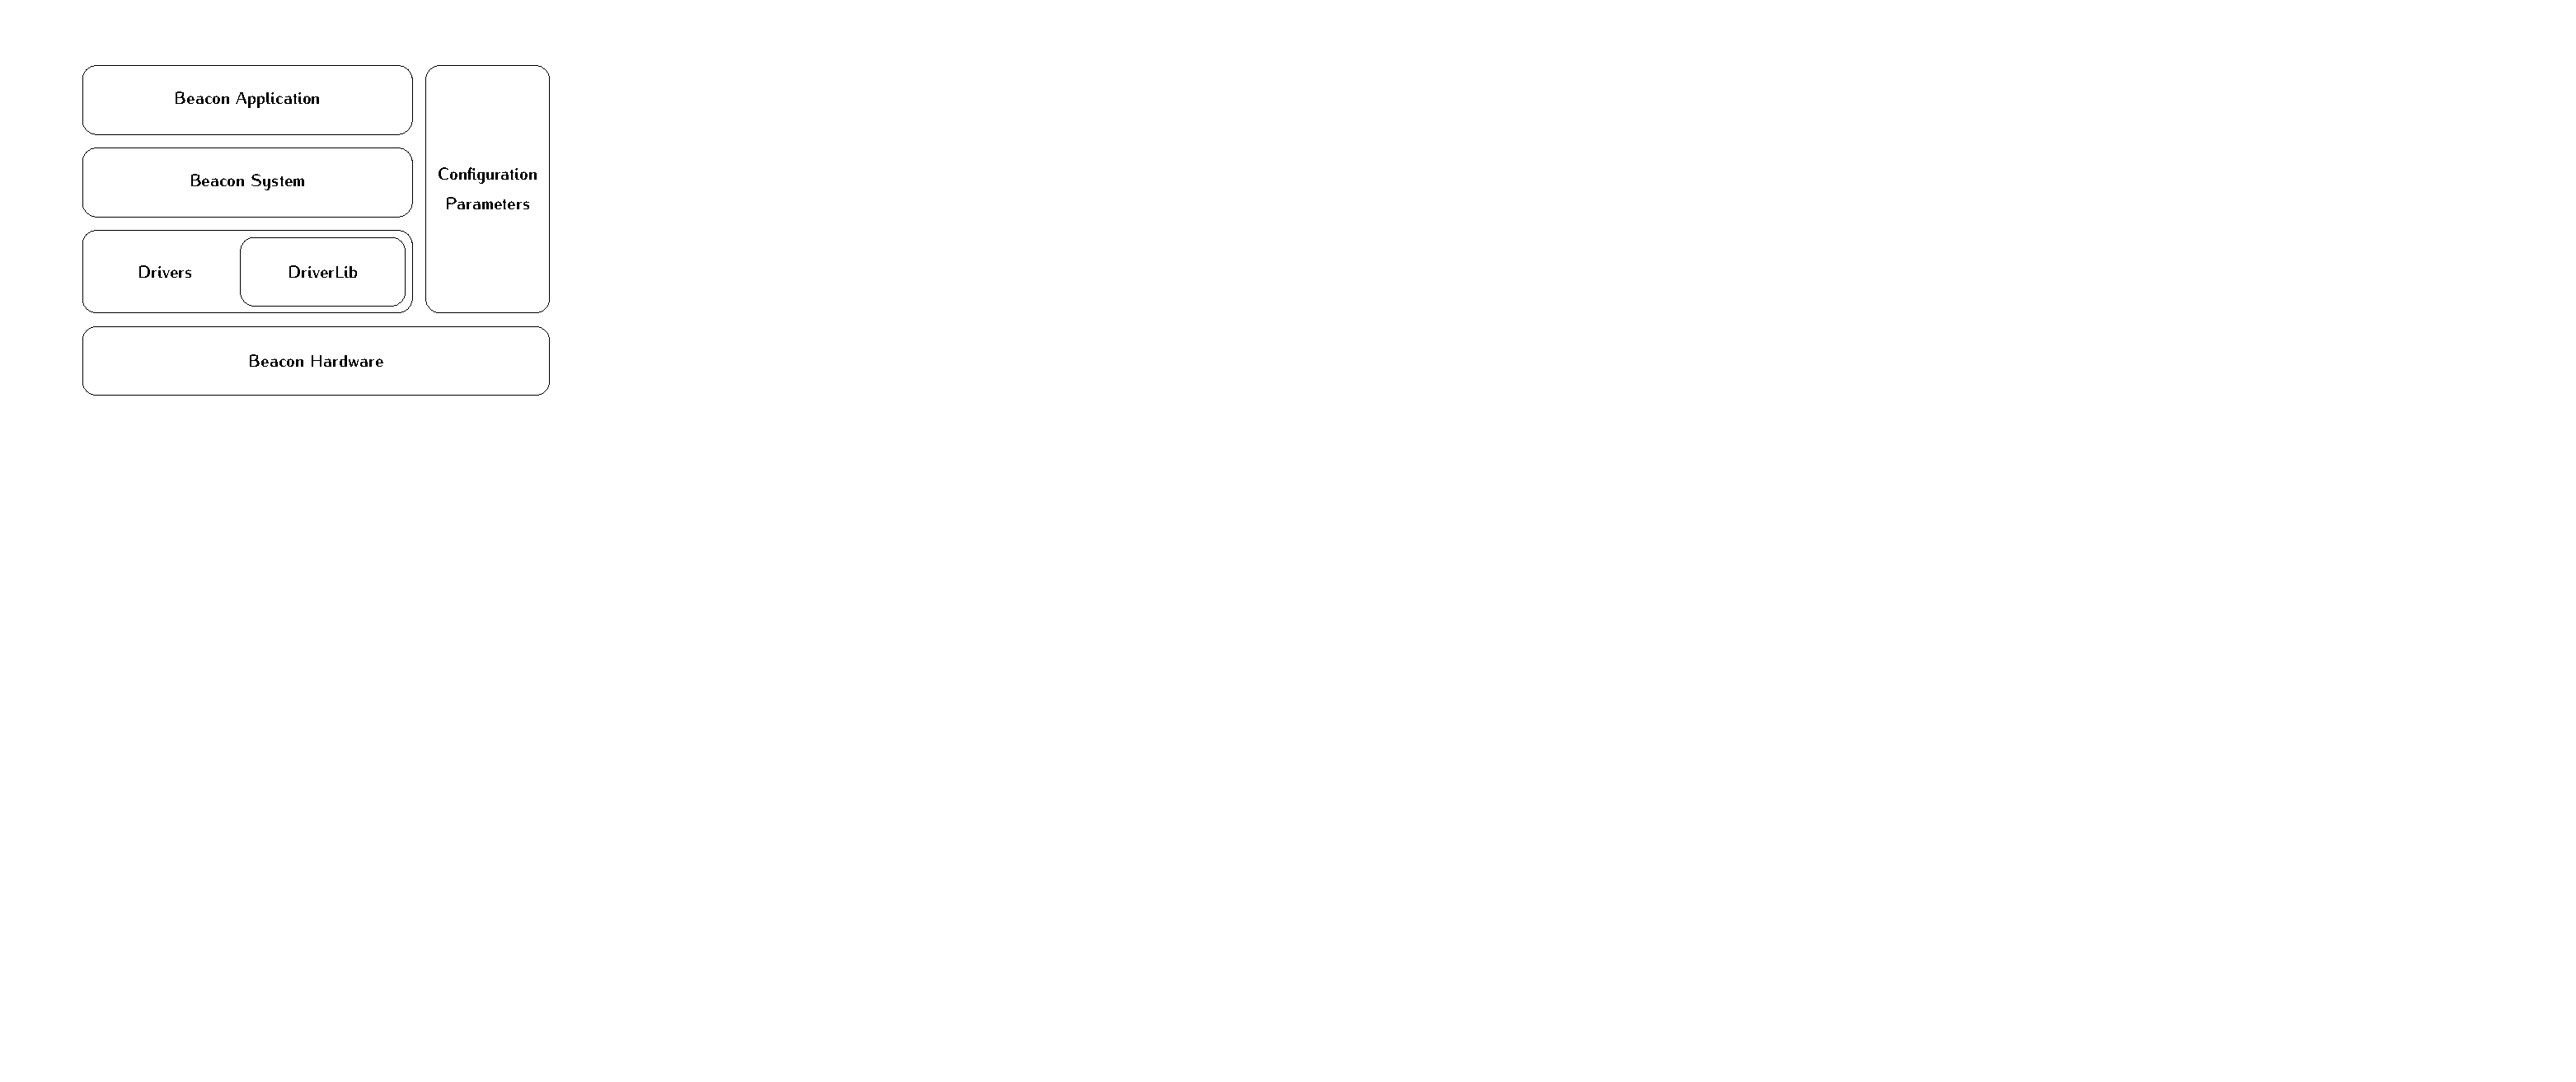
\includegraphics[width=0.5\textwidth]{figures/beacon_software_layers.pdf}
		\caption{Beacon software stack-up.}
		\label{fig:beacon-software-layers}
	\end{center}
\end{figure}

It is composed by five layers:

\begin{itemize}
    \item Hardware layer: All the TTC hardware (MSP430F6659 and the RF4463F30).
    \item Drivers layer: The software to make the interface with the hardware (Internal peripherals of the uC, the radio module and the antenna module).
    \item System layer: General usage functions and resources of the beacon system (like data structures, power management, etc.).
    \item Application layer: The main beacon software, where all the tasks were implemented.
\end{itemize}

\section{Flowcharts}

\subsection{Main}

\begin{figure}[!h]
	\begin{center}
		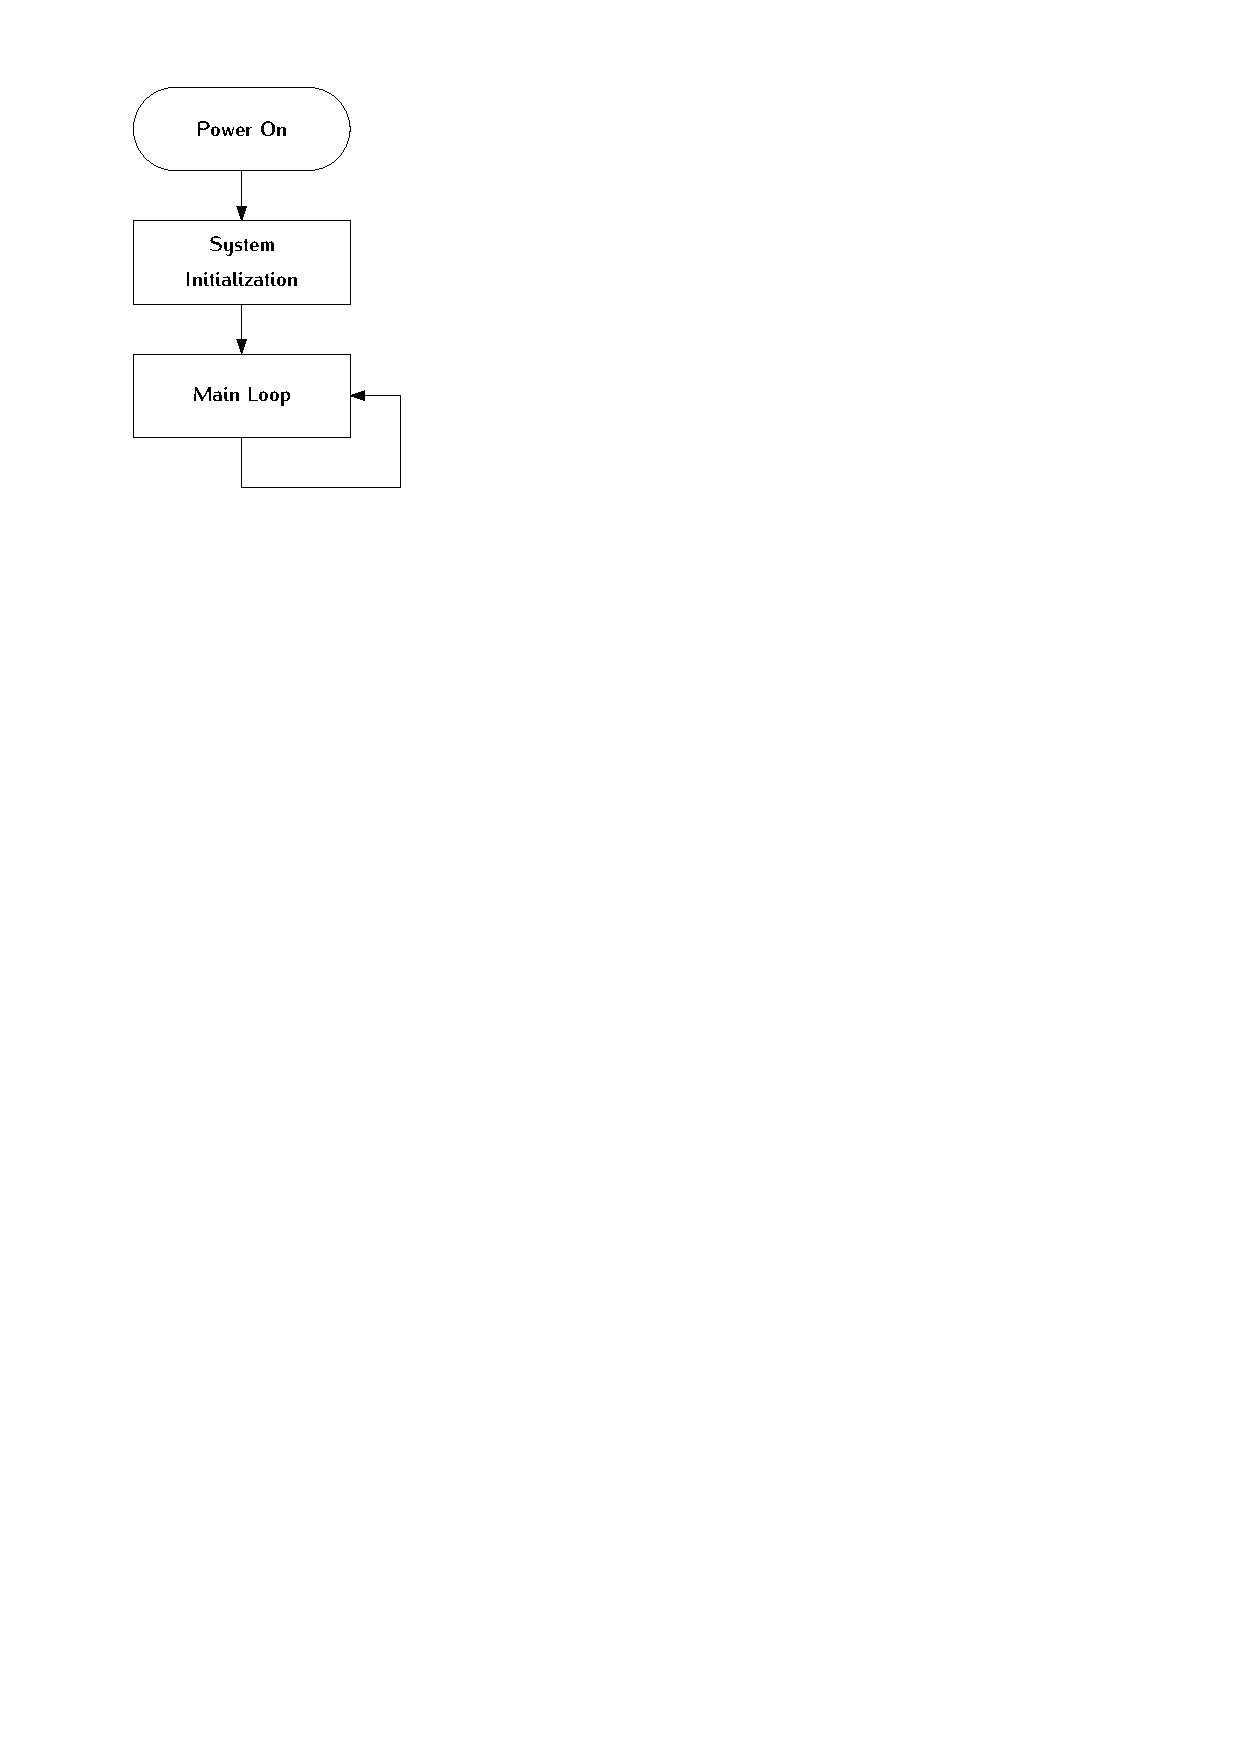
\includegraphics[width=0.25\textwidth]{figures/beacon_main_flowchart.pdf}
		\caption{Main flowchart of the beacon software.}
		\label{fig:beacon-main-flowchart}
	\end{center}
\end{figure}

\subsection{Initialization}

\begin{figure}[!h]
	\begin{center}
		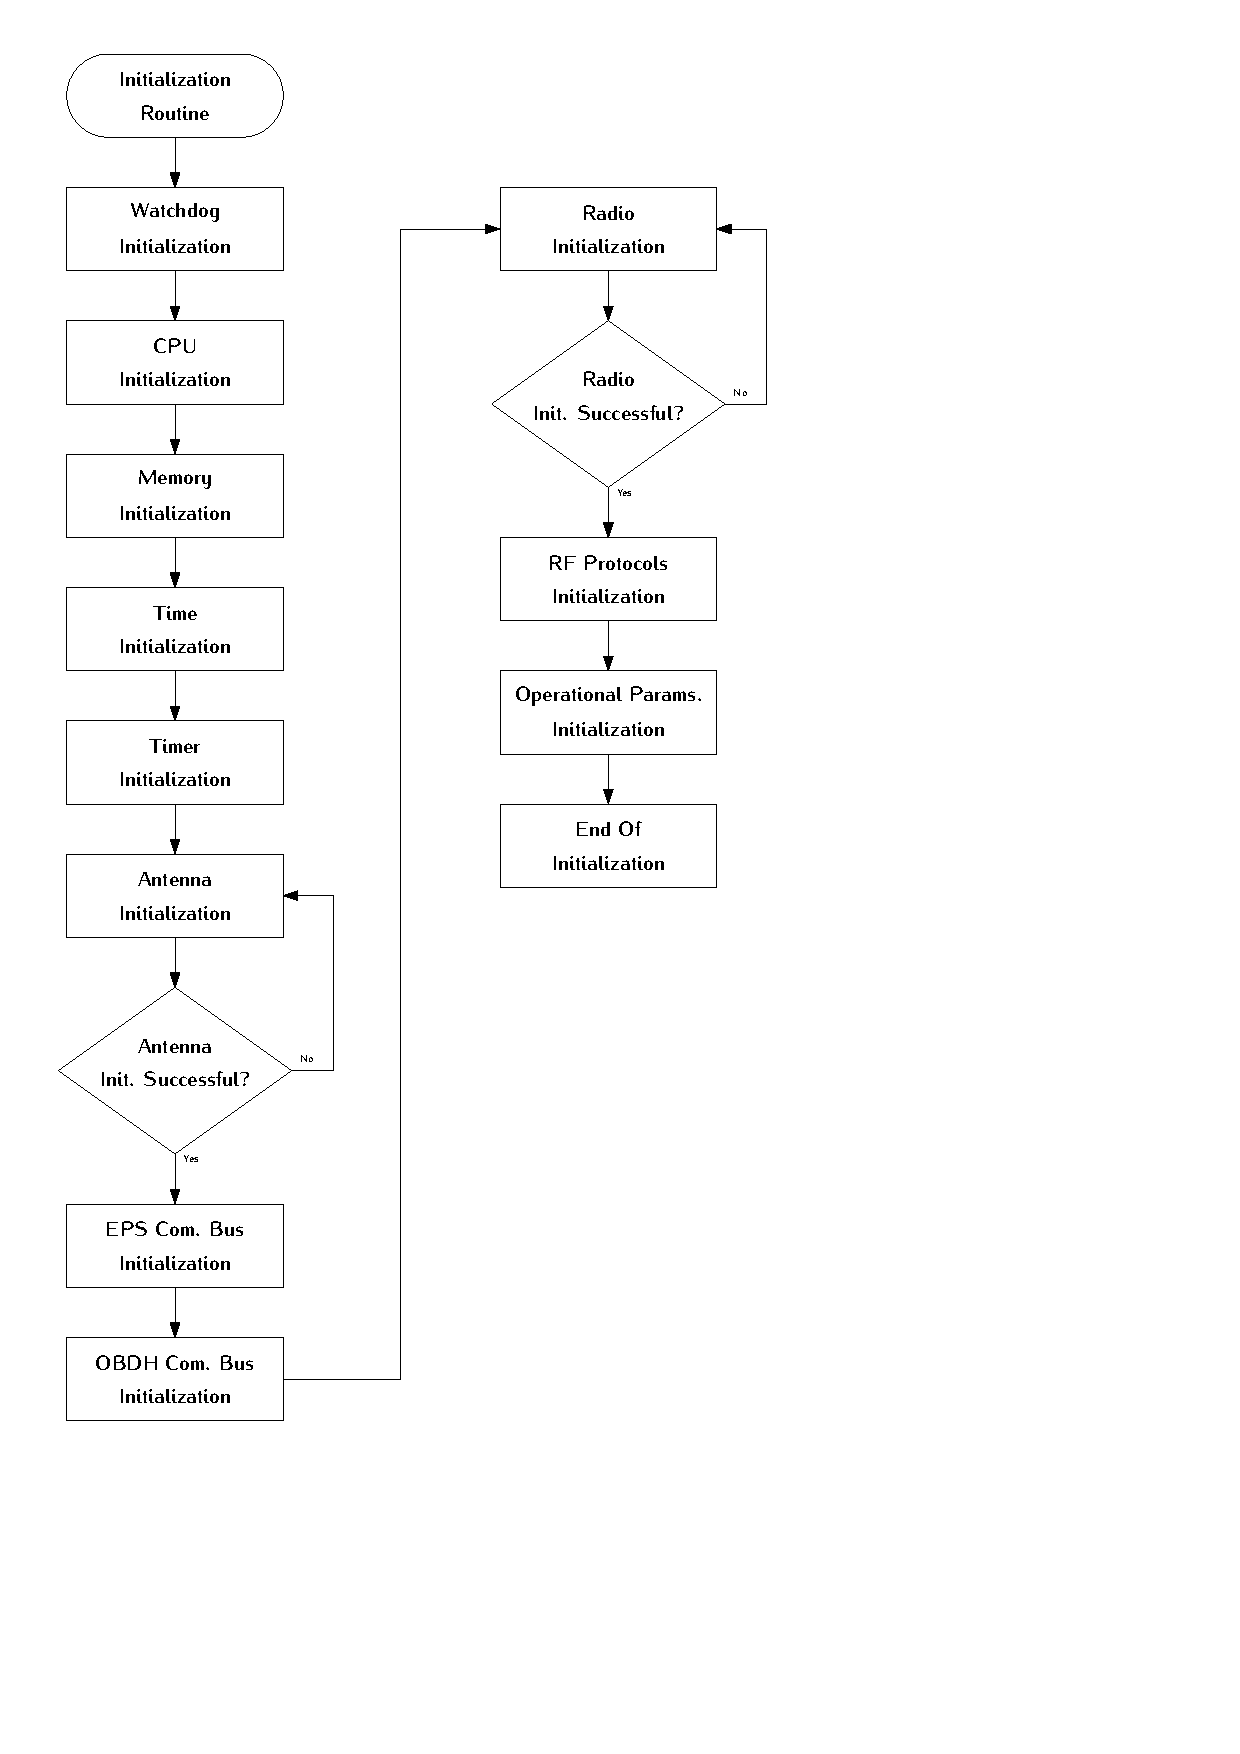
\includegraphics[width=0.75\textwidth]{figures/beacon_init_flowchart.pdf}
		\caption{Flowchart of the beacon initialization.}
		\label{fig:beacon-init-flowchart}
	\end{center}
\end{figure}

\subsubsection{Watchdog}

The watchdog is initialized using the ACLK as clock source and a 512k clock divider (generating a 16 second watchdog). The counter starts right after the initialization.

\subsubsection{CPU}

For the CPU configuration, the core voltage is setted to level 2 (required for a clock between 12 and 20 MHz). The DCO FLL reference is setted to REF0 (with the clock divider equal to 1). The ACLK clock is setted to be equal to REF0 (same as DCO, clock divider equal to 1). The SMCLK reference is setted to be the DCO, but with a divider factor equal to 4.

So, the final configuration is: MCLK = 16 MHz, SMCLK = 4 MHz and ACLK = 32,768 kHz.

\subsubsection{Memory}

UNDER DEVELOPMENT.

\subsubsection{Time}

During the time initialization, the last value stored in the memory is loaded and the counter continues from it value, preventing the lost of time reference after a system reboot or fault.

\subsubsection{Timer}

For the system time, a 1 second timer is used (using the timer interruption to increment a second counter variable, 32-bit unsigned integer). This counting starts from the last value stored into the memory.

\subsubsection{Antenna}

UNDER DEVELOPMENT.

\subsubsection{EPS Communication Bus}

The EPS communication bus (UART) is configured at a transfer rate of 4800 bps, no parity bit, LSB first and one stop bit. The clock source of this UART bus is the SMCLK. The EPS queue is also initialized.

\subsubsection{OBDH Communication Bus}

The same occurs for the OBDH communication bus (SPI): the transfer rate is 2400 bps and the endianness is MSB first. The OBDH queue is also initialized.

\subsubsection{Radio}

During the initialization of the radio, it is reseted and all the configuration parameters are transfered to the radio module. More informations about this process can be found in the radio IC documentation.

\subsubsection{RF Protocols}

The NGHam, AX.25 and the FSP protocols also need an initialization, to set internal variables and counters.

\subsection{ISRs}

\nomenclature{\textbf{ISR}}{Interruption Service Routine.}

\subsubsection{OBDH and EPS Communication}

The flowchart of the interruption service routine (ISR) of the OBDH communication can be seen in the figure \ref{fig:beacon-obdh-isr-flowchart}. Basically, when a new byte arrives, it is pushed to a queue (if it isn't full), and periodically, the OBDH communication task process these new bytes (taking out the bytes from the queue).

The flowchart of the interruption service routine (ISR) of the EPS communication can be seen in the figure \ref{fig:beacon-eps-isr-flowchart}. It's operation is equal to the OBDH communication ISR.

\begin{figure}[!h]
	\begin{center}
		\subfigure[OBDH communication ISR flowchart.\label{fig:beacon-obdh-isr-flowchart}]{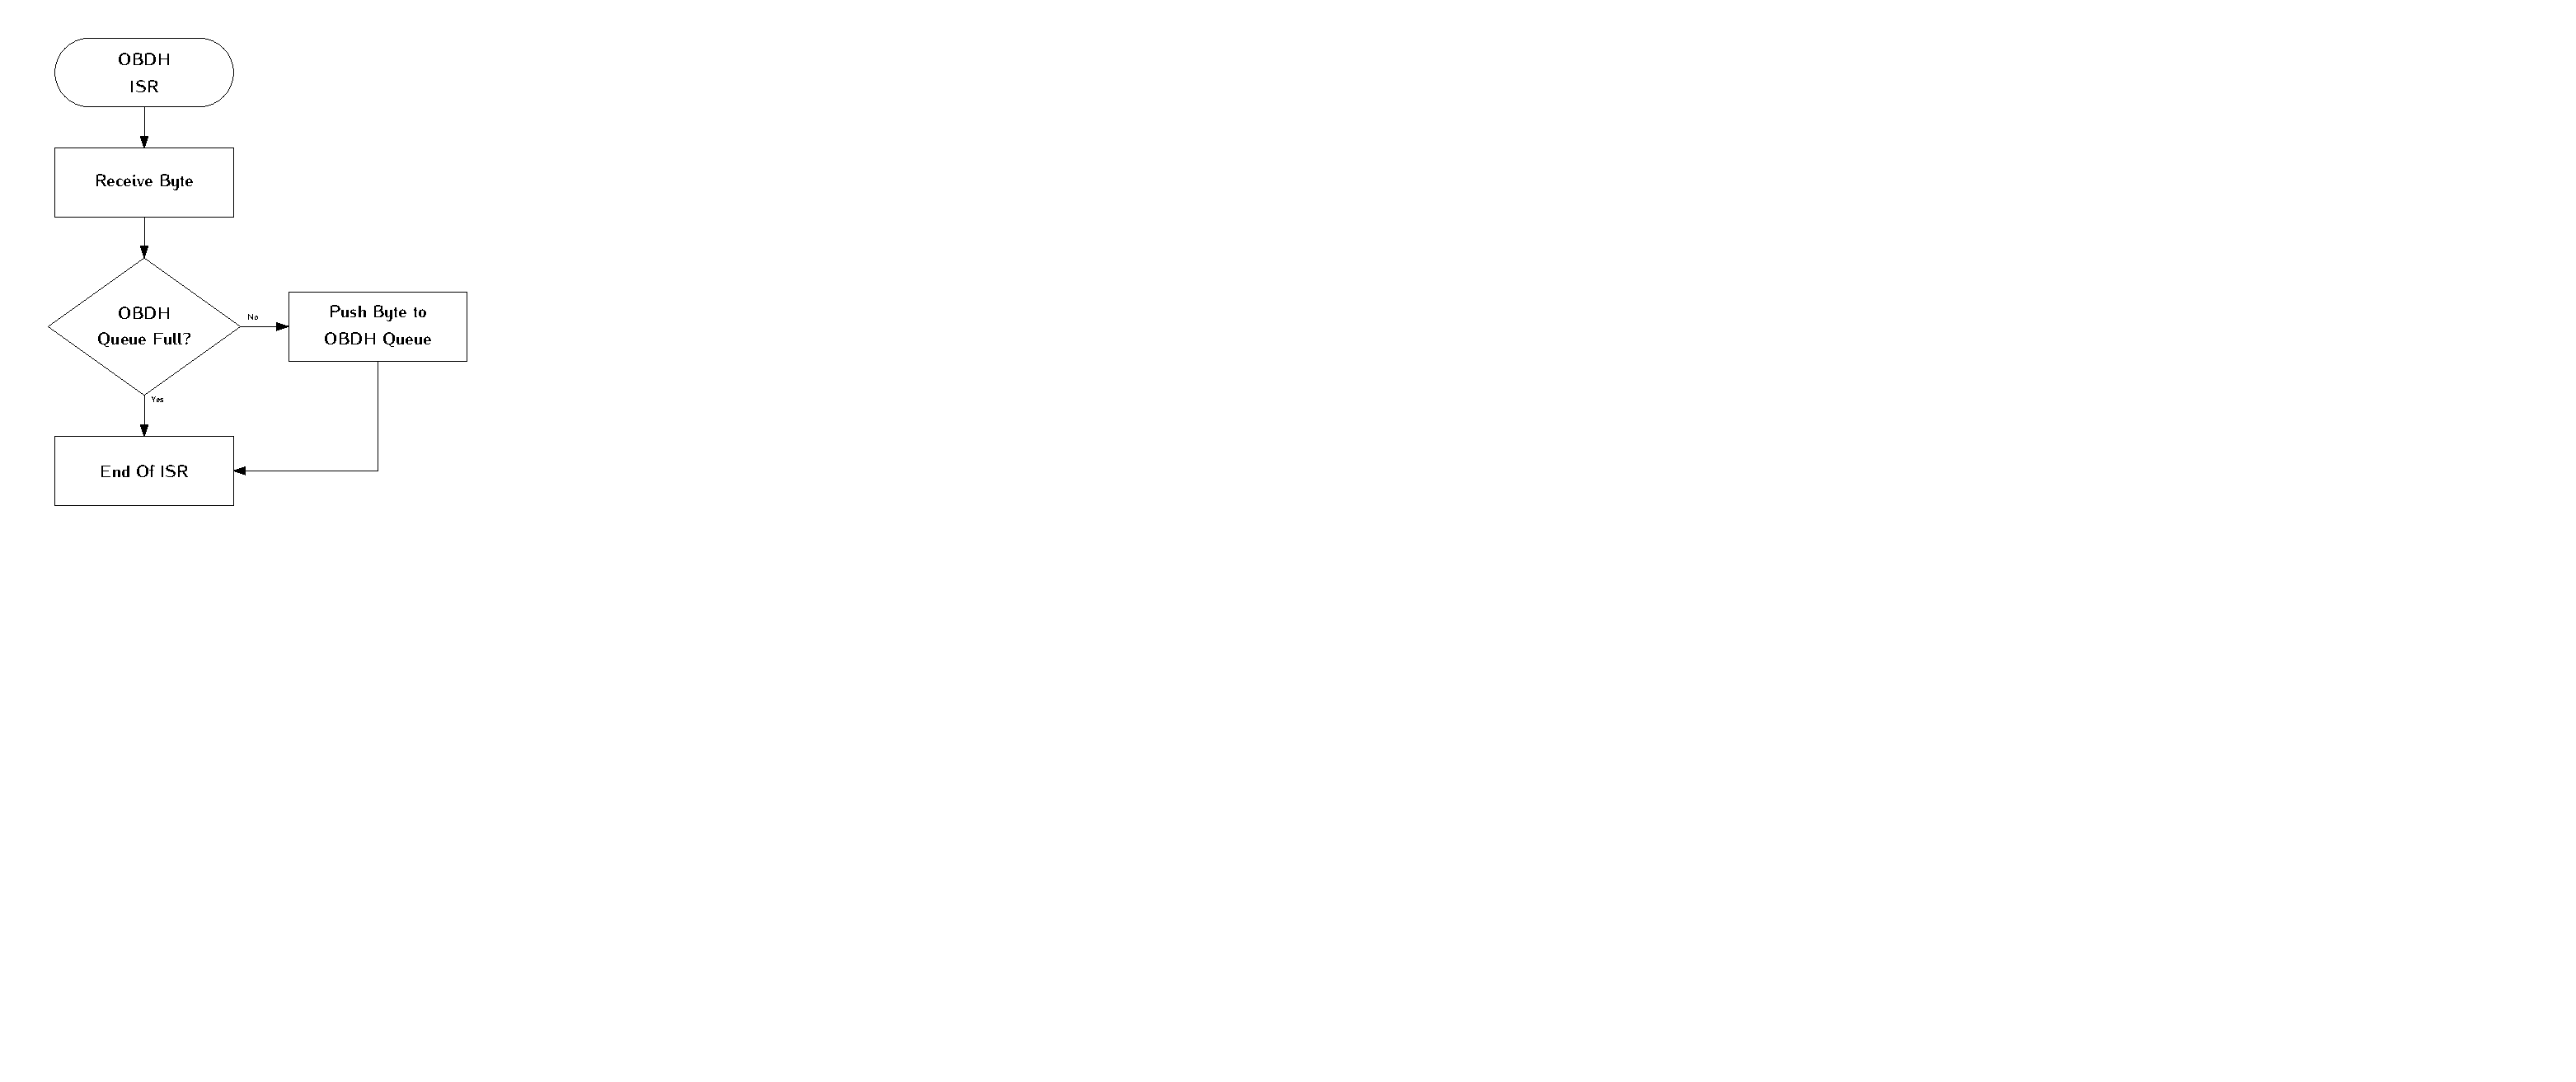
\includegraphics[width=0.4\textwidth]{figures/beacon_obdh_isr_flowchart.pdf}}
		\qquad
		\subfigure[EPS communication ISR flowchart.\label{fig:beacon-eps-isr-flowchart}]{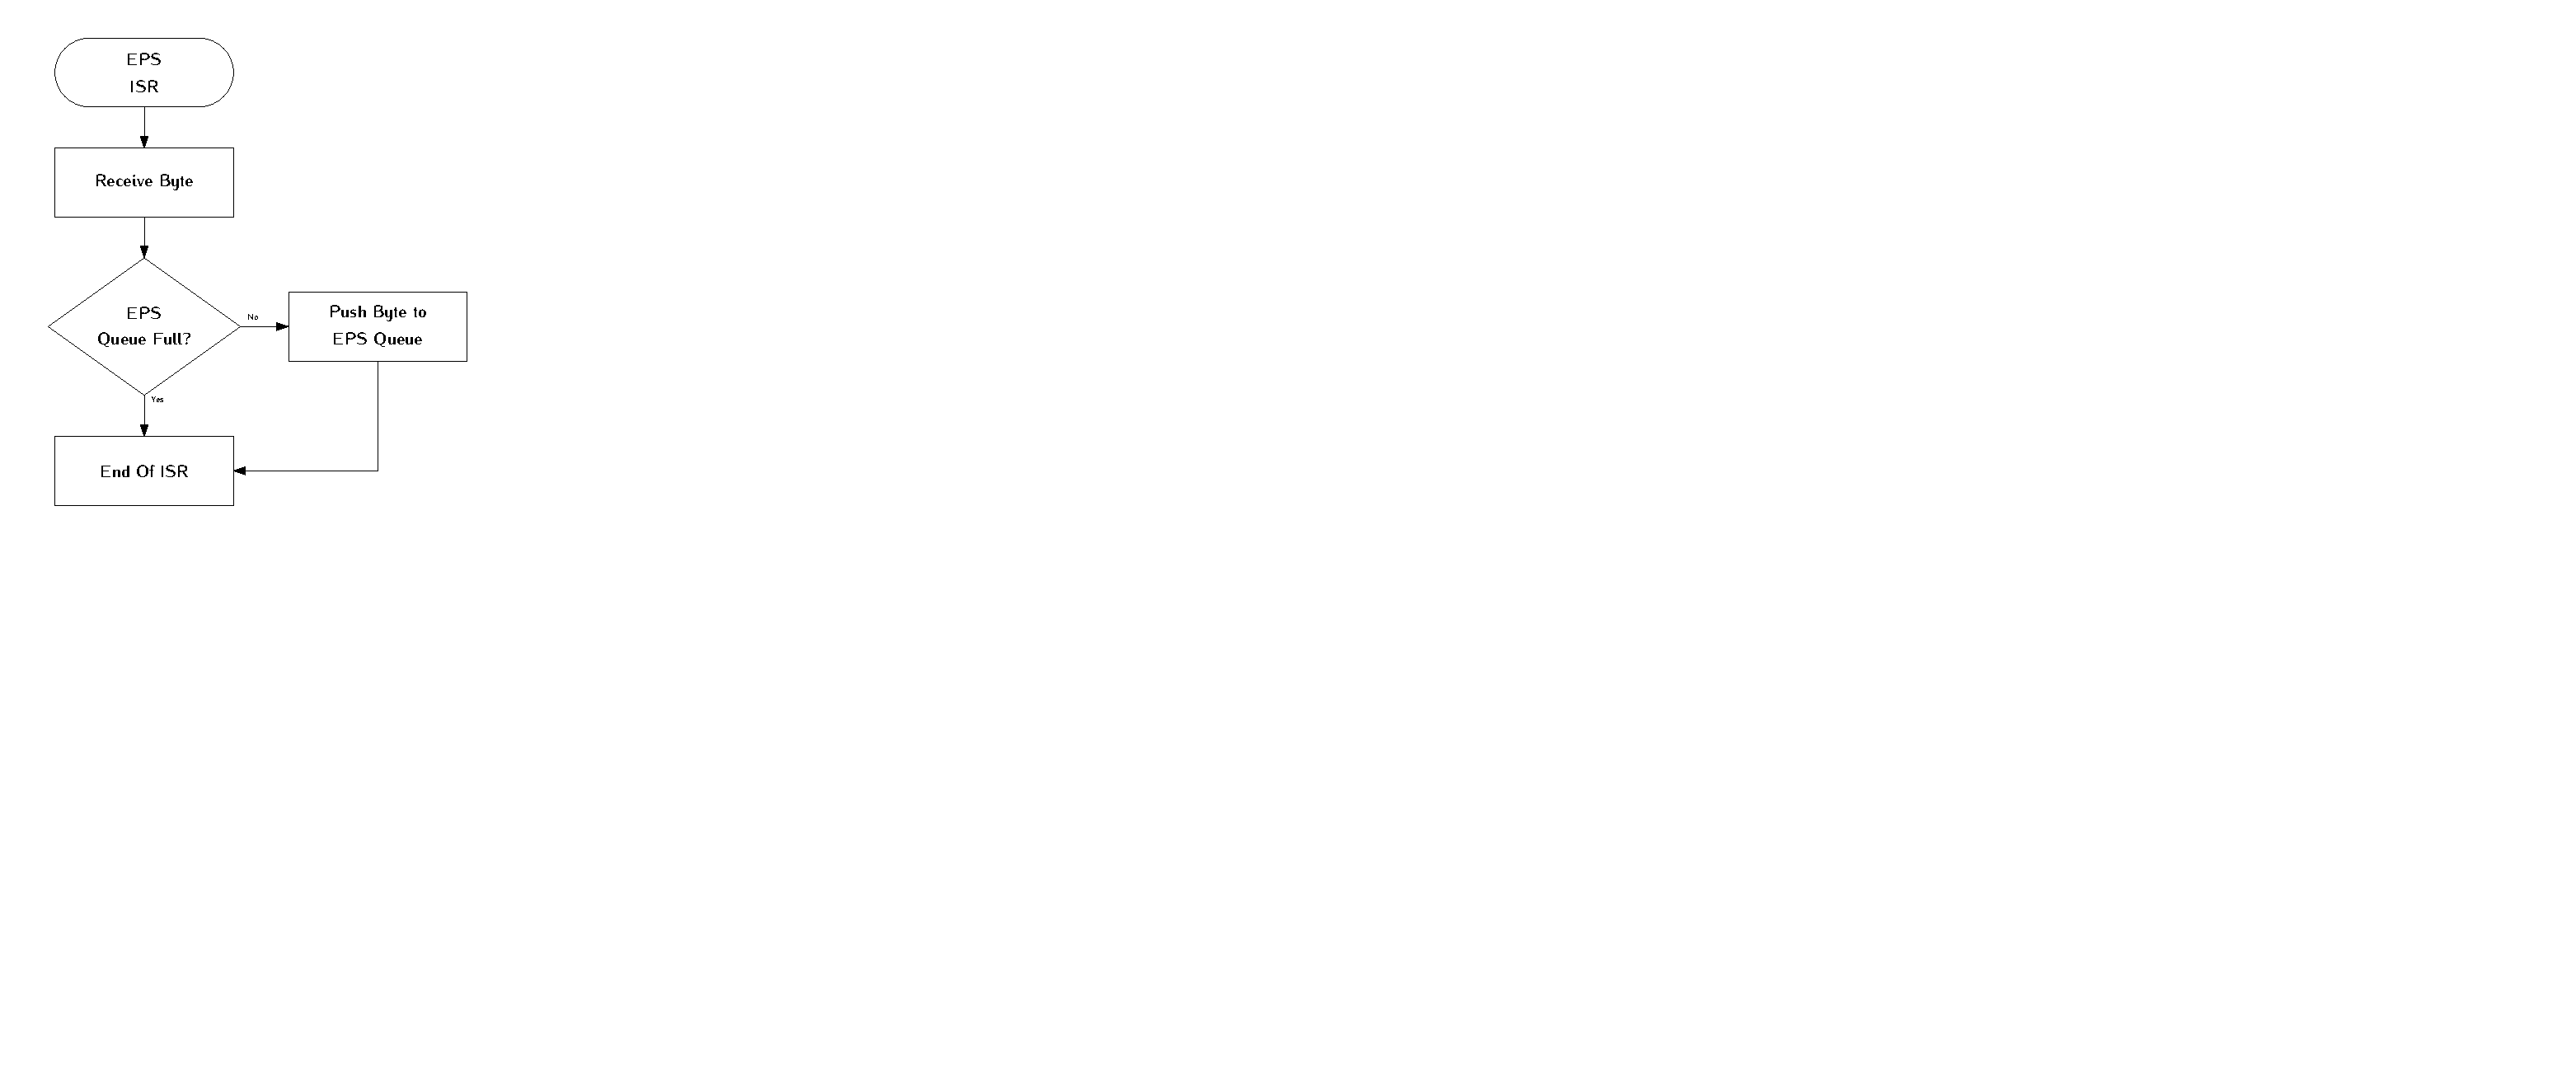
\includegraphics[width=0.4\textwidth]{figures/beacon_eps_isr_flowchart.pdf}}
		\caption{OBDH and EPS modules comunication ISRs routines.}
		\label{fig:obdh-eps-isr-flowchart}
	\end{center}
\end{figure}

\section{Operation Modes}

There are three operation modes in the beacon software:

\begin{itemize}
    \item DEBUG MODE: In this mode, the operation of the beacon is described through an UART port. At every operation, a message describing what is happening is transmitted to the debug UART port.
    \item TEST MODE: In this mode, the antenna deployment routines are not executed. This is the main mode to use during the satellite integration tests.
    \item FLIGHT MODE: This is the mode to use in flight, with all the available resources enabled.
\end{itemize}

The selection of the operation mode can be done using the ``BEACON\_MODE" variable in the ``config.h" file.

\section{Tasks}

In the table \ref{tab:sw_tasks}, the beacon tasks are listed with a brief description and its period of execution.

\begin{table}[!h]
	\begin{center}
		\begin{tabular}{L{0.2\textwidth} C{0.4\textwidth} C{0.3\textwidth}}
			\toprule[1.5pt]
			\textit{Task} & \textit{Description} & \textit{Period} \\
			\midrule
			System initialization & Submodules initialization (CPU, memory, radio, etc.) & Aperiodic (Executed only at initializations) \\
			Antenna deployment & 145 MHz band antenna deployment after the satellite launch & Aperiodic (Executed once) \\
			NGHam packet transmission & Transmission of the beacon packets with a basic telemetry data using the NGHam protocol & 10, 20 or 30 seconds (EPS energy level dependent) \\
			AX.25 packet transmission & Transmission of the beacon packets with a basic telemetry data using the AX.25 protocol & 10, 20 or 30 seconds (EPS energy level dependent) \\
			OBDH data processing & The OBDH module can send telemetry data or commands & Aperiodic (OBDH module dependent) \\
			EPS data processing & The EPS modules sends telemetry data & Aperiodic (EPS module dependent) \\
			Radio data processing & Processing of an incoming packet from the beacon radio & Aperiodic (Only when the OBDH fails and an hibernation is required) \\
			Beacon radio reception activation & When a critical failure occur in the OBDH module, the beacon activates its reception between the beacon transmissions & Aperiodic (Only when the OBDH module fails) \\
			Radio reset & Beacon radio reset & 10 minutes \\
			Beacon reset & Beacon system reset & 12 hours \\
			\bottomrule[1.5pt]
		\end{tabular}
		\caption{Beacon software tasks.}
		\label{tab:sw_tasks}
	\end{center}
\end{table}

\section{Packets Payload}

In the normal satellite operation, the beacon packets contains the data from the table \ref{tab:beacon-normal-payload}.

\begin{table}[!h]
	\begin{center}
		\begin{tabular}{lc}
			\toprule[1.5pt]
			\textit{Information} & \textit{Length (Bytes)} \\
			\midrule
			Satellite ID: ``FLORIPASAT" & 10 \\
			Batteries voltages & 4 \\
			Batteries temperatures & 6 \\
			Total charge of batteries & 2 \\
			Solar panels currents & 12 \\
			Solar panels voltages & 6 \\
			Overall status of the satellite & 2 \\
			Accelerometer and gyroscope & 12 \\
			Time since boot & 4 \\
			Number of OBDH module resets since launch & 2 \\
			\bottomrule[1.5pt]
		\end{tabular}
		\caption{Normal content of the beacon packets.}
		\label{tab:beacon-normal-payload}
	\end{center}
\end{table}

If a fault on the OBDH module occurs, only the EPS data are transmitted, the contents of this kind of packet can be seen in the table \ref{tab:beacon-without-obdh-payload}.

\begin{table}[!h]
	\begin{center}
		\begin{tabular}{lc}
			\toprule[1.5pt]
			\textit{Information} & \textit{Length (Bytes)} \\
			\midrule
			Satellite ID: ``FLORIPASAT" & 10 \\
			Batteries voltages & 4 \\
			Batteries temperatures & 6 \\
			Total charge of batteries & 2 \\
			Solar panels currents & 12 \\
			Solar panels voltages & 6 \\
			Energy level & 1 \\
			\bottomrule[1.5pt]
		\end{tabular}
		\caption{Content of the beacon packets with a fault in the OBDH module.}
		\label{tab:beacon-without-obdh-payload}
	\end{center}
\end{table}

If a fault occurs in the OBDH and the EPS modules, only the satellite ID is transmitted. It can be seen in the table \ref{tab:beacon-without-eps-payload}.

\begin{table}[!h]
	\begin{center}
		\begin{tabular}{lc}
			\toprule[1.5pt]
			\textit{Information} & \textit{Length (Bytes)} \\
			\midrule
			Satellite ID: ``FLORIPASAT" & 10 \\
			\bottomrule[1.5pt]
		\end{tabular}
		\caption{Content of the beacon packets with a fault in the OBDH and EPS modules.}
		\label{tab:beacon-without-eps-payload}
	\end{center}
\end{table}

The decodification of the packets data are done automatically by the GRS software.

\section{USCIs Configuration}

\begin{table}[!h]
	\begin{center}
		\begin{tabular}{lcc}
			\toprule[1.5pt]
			\textit{MSP Interface} & \textit{Mode} & \textit{Connected Components} \\
			\midrule
			USCI\_A0 & UART RX & EPS Bus \\
			USCI\_A0 & UART TX & Packets transmission (Only for tests) \\
			USCI\_A1 & UART TX/RX & Debug \\
			USCI\_A2 & SPI Slave & OBDH Bus \\
			USCI\_B0 & SPI Master & Beacon transceiver \\
			USCI\_B2 & $I^{2}C$ Master & Antenna bus  \\
			\bottomrule[1.5pt]
		\end{tabular}
		\caption{USCIs configuration of the beacon microcontroller.}
		\label{tab:beacon-uc-usci-config}
	\end{center}
\end{table}

\section{Timers}

\begin{table}[!h]
	\begin{center}
		\begin{tabular}{lccc}
			\toprule[1.5pt]
			\textit{Timer Interface} & \textit{Mode} & \textit{Period} & \textit{Function} \\
			\midrule
			TIMER\_A1 & Continuous-Compare & 1 s & Time Control \\
			\bottomrule[1.5pt]
		\end{tabular}
		\caption{Timers configuration of the beacon microcontroller.}
		\label{tab:beacon-uc-timers-config}
	\end{center}
\end{table}
